\documentclass[%
reprint,
superscriptaddress,
groupedaddress,
superscriptaddress,
onecolumn,
10pt
]{revtex4-2}
\usepackage[margin=2cm]{geometry}
\usepackage{graphicx,braket,bm,hyperref,amsmath,amssymb}

\begin{document}

\title{Quantum criticality in a Kondo-Mott lattice model}

\author{Abhirup Mukherjee}
\author{Siddhartha Lal}

\date{\today}

\maketitle
\section{Impurity Model}
\begin{equation}\begin{aligned}
	H_\text{aux}({\bf r}_d) = H^{(0)} + H_f({\bf r}_d) + H_c({\bf r}_d) + H_{fc}({\bf r}_d)~,
\end{aligned}\end{equation}
\begin{equation}\begin{aligned}
	H^{(0)} =& -t_f\sum_{\braket{i,j},\sigma}\left(f^\dagger_{i,\sigma}f_{j,\sigma} + \text{h.c.}\right) -t\sum_{\braket{i,j},\sigma}\left(c^\dagger_{i,\sigma}c_{j,\sigma} + \text{h.c.}\right) - \mu\sum_{i,\sigma}\left(f^\dagger_{i,\sigma}f_{i,\sigma} + c^\dagger_{i,\sigma}c_{i,\sigma}\right) ~,\\
	H_f({\bf r}_d) =& V_f\sum_{Z \in \text{NN}}\sum_{\sigma}\left(f^\dagger_{{\bf r}_d,\sigma} f_{Z,\sigma} + \text{h.c.}\right) + \epsilon_f \sum_\sigma f^\dagger_{{\bf r}_d,\sigma}f_{{\bf r}_d,\sigma} + U_f f^\dagger_{{\bf r}_d,\uparrow}f_{{\bf r}_d,\uparrow} f^\dagger_{{\bf r}_d,\downarrow}f_{{\bf r}_d,\downarrow} \\
				   &+ J_f\sum_{Z \in \text{NN}}\sum_{\alpha,\beta}{\bf S}_f({\bf r}_d) \cdot {\boldsymbol{\sigma}}_{\alpha\beta}f^\dagger_{Z,\alpha}f_{Z,\beta} - \frac{W_f}{2} \sum_{Z \in \text{NN}}\left(f^\dagger_{Z,\uparrow}f_{Z,\uparrow} - f^\dagger_{Z,\downarrow}f_{Z,\downarrow} \right)^2~,\\
	H_c({\bf r}_d) =& - \frac{W}{2}\left(c^\dagger_{{\bf r}_d,\uparrow}c_{{\bf r}_d,\uparrow} - c^\dagger_{{\bf r}_d,\downarrow}c_{{\bf r}_d,\downarrow} \right)^2~,\\
	H_{fc}({\bf r}_d) =& J\sum_{\alpha,\beta}{\bf S}_f({\bf r}_d) \cdot {\boldsymbol{\sigma}}_{\alpha\beta}c^\dagger_{{\bf r}_d,\alpha}c_{{\bf r}_d,\beta} + V \left(f^\dagger_{{\bf r}_d,\sigma} c_{{\bf r}_d,\sigma} + \text{h.c.}\right)~,\\
\end{aligned}\end{equation}

\section{Tiling reconstruction}
\begin{equation}\begin{aligned}
	H_\text{tiled} =& \sum_{{\bf r}_d}H_\text{aux}({\bf r}_d) - (N-1) H^{(0)} \\
	=& \sum_{\braket{i,j},\sigma}\left[-t_f\left(f^\dagger_{i,\sigma}f_{j,\sigma} + \text{h.c.}\right) -t\left(c^\dagger_{i,\sigma}c_{j,\sigma} + \text{h.c.}\right)\right] + \tilde J \sum_{\braket{i,j}}{\bf S}_f(i) \cdot {\bf S_f}(j) + J\sum_i {\bf S}_f(i)\cdot {\bf S}_c(i) - U\sum_i \left(f^\dagger_{i,\uparrow}f_{i,\uparrow} - f^\dagger_{i,\downarrow}f_{i,\downarrow}\right)^2 \\
	 &- \mu N
\end{aligned}\end{equation}

\section{Coupling renormalisation group flows}
Off-diagonal terms:
\begin{equation}\begin{aligned}
	H_{X, f} &= \frac{1}{2}\sum_{{\bf q},{\bf k},\sigma}J_f({\bf k},{\bf q}) S_f^\sigma \left(f^\dagger_{{\bf q},-\sigma}f_{{\bf k},\sigma} + f^\dagger_{{\bf k},-\sigma}f_{{\bf q},\sigma}\right) + \frac{1}{2}\sum_{{\bf q},{\bf k},\sigma}J_f({\bf k},{\bf q}) \sigma S_f^z \left(f^\dagger_{{\bf q},\sigma}f_{{\bf k},\sigma} + f^\dagger_{{\bf k},\sigma}f_{{\bf q},\sigma}\right)~,\\
	H_{X, c} &= \frac{1}{2}J\sum_{{\bf q},{\bf k},\sigma} S_f^\sigma \left(c^\dagger_{{\bf q},-\sigma}c_{{\bf k},\sigma} + c^\dagger_{{\bf k},-\sigma}c_{{\bf q},\sigma}\right) + \frac{1}{2}J\sum_{{\bf q},{\bf k},\sigma} \sigma S_f^z \left(c^\dagger_{{\bf q},\sigma}c_{{\bf k},\sigma} + c^\dagger_{{\bf k},\sigma}c_{{\bf q},\sigma}\right)~.
\end{aligned}\end{equation}

\subsection{Intra-layer processes}
\begin{equation}\begin{aligned}
	\Delta J_f^{(j)}\left({\bf k}_1, {\bf k}_2\right) &= -\sum_{{\bf q} \in \text{PS}} \left(J_f^{(j)}\left({\bf k}_2,{\bf q}\right) J_f^{(j)}\left({\bf q},{\bf k}_1\right) + 4J_f^{(j)}\left({\bf q}, {\boldsymbol \pi} + {\bf q}\right) W_{{\boldsymbol \pi} + {\bf q}, {\bf k}_2, {\bf k}_1, {\bf q}}\right) G_f(\omega, {\bf q})~,\\
	\Delta J^{(j)} &= - \rho(\varepsilon_j)\Delta \varepsilon\cdot\left[\left(J^{(j)}\right)^2 + 4WJ^{(j)}\right]~G(\omega, {\bf q})~,
\end{aligned}\end{equation}
where \({\bf \bar q} = {\boldsymbol \pi} + {\bf q}\) is the charge conjugate partner of \({\bf q}\), and the propagators \(G_f\) and \(G\) are defined as
\begin{equation}\begin{aligned}\label{propagators}
	G_f(\omega,{\bf q}) &= \frac{1}{2}\left[\left(\omega - \frac{1}{2}\left(|\varepsilon_f({\bf q})| - \mu\right) + J^{(j)}_f\left({\bf q},{\bf q}\right)/4 + W_f({\bf q})/2 - \epsilon_f\right)^{-1} + \left(\omega - \frac{1}{2}\left(|\varepsilon_f({\bf q})| + \mu\right) + J^{(j)}_f\left({\bf q},{\bf q}\right)/4 + W_f({\bf q})/2 - \epsilon_f\right)^{-1}\right] ~,\\
	G(\omega,{\bf q}) &= \frac{1}{2}\left[\left(\omega - \frac{1}{2}|\varepsilon({\bf q})| + J^{(j)}/4 + W/2 + \mu/2\right)^{-1} + \left(\omega - \frac{1}{2}|\varepsilon({\bf q})| + J^{(j)}/4 + W/2 - \mu/2\right)^{-1}\right] ~.
\end{aligned}\end{equation}


\subsection{Inter-layer processes}
Processes that start from configurations in which \({\bf q}\) is occupied:
\begin{equation}\begin{aligned}
	P_1 = \frac{1}{8}\sum_{{\bf q},{\bf k},{\bf k}_1, {\bf k}_2,\sigma,\sigma^\prime} J_f^{(j)}({\bf q},{\bf k}) S_f^\sigma f^\dagger_{{\bf q},-\sigma}f_{{\bf k},\sigma} ~ G_f(\omega, {\bf q}, {\bf k}) ~ J^{(j)} S_f^z \sigma^\prime c^\dagger_{{\bf k}_1,\sigma^\prime}c_{{\bf k}_2,\sigma^\prime} ~ G_f(\omega, {\bf q}, {\bf k}) ~ J_f^{(j)}({\bf q},{\bf k}) S_f^{-\sigma} f^\dagger_{{\bf k},\sigma}f_{{\bf q},-\sigma}~,
\end{aligned}\end{equation}
where the propagator \(G_f(\omega, {\bf q}, {\bf k})\) for the excitations is a generalisation of eq.~\ref{propagators}:
\begin{equation}\begin{aligned}
	G_f(\omega, {\bf q}, {\bf k}) &= \left(\omega - \frac{1}{2}|\varepsilon_f({\bf q})| - \frac{1}{2}|\varepsilon_f({\bf k})| + J^{(j)}_f\left({\bf q},{\bf q}\right)/4 + J^{(j)}_f\left({\bf k},{\bf k}\right)/4 + W_f({\bf q})/2 + W_f({\bf k})/2 - \epsilon_f\right)^{-1} ~,\\
\end{aligned}\end{equation}

Using \(S^\sigma S^z = -\frac{\sigma}{2}S^\sigma\) and \(S^\sigma S^{-\sigma} = \frac{1}{2} + \sigma S^z\), we get
\begin{equation}\begin{aligned}
	P_1 &= \sum_{{\bf k}_1, {\bf k}_2,\sigma,\sigma^\prime} \frac{-\sigma^\prime}{16} \left(\frac{\sigma}{2} + S_f^z\right) c^\dagger_{{\bf k}_1,\sigma^\prime}c_{{\bf k}_2,\sigma^\prime} ~  J^{(j)} \sum_{{\bf q} \in \text{PS} ,{\bf k} \in \text{HS}}\left(J_f^{(j)}({\bf q},{\bf k})\right)^2 G^2_f(\omega, {\bf q}, {\bf k})\\
		&= -\frac{1}{8}\sum_{{\bf k}_1, {\bf k}_2,\sigma^\prime} \sigma^\prime~S_f^z c^\dagger_{{\bf k}_1,\sigma^\prime}c_{{\bf k}_2,\sigma^\prime} ~  J^{(j)} \sum_{{\bf q} \in \text{PS} ,{\bf k} \in \text{HS}}\left(J_f^{(j)}({\bf q},{\bf k})\right)^2 G^2_f(\omega, {\bf q}, {\bf k})~.
\end{aligned}\end{equation}

Another process can be conceived with similar starting configuration but where the loop momenta are on the \(c-\)plane:
\begin{equation}\begin{aligned}
	P_2 = \frac{1}{8}\sum_{{\bf q},{\bf k},{\bf k}_1, {\bf k}_2,\sigma,\sigma^\prime} J^{(j)} S_f^\sigma c^\dagger_{{\bf q},-\sigma}c_{{\bf k},\sigma} ~ \tilde \tilde G(\omega, {\bf q}, {\bf k}) ~ J^{(j)}({\bf k}_1,{\bf k}_2) S_f^z \sigma^\prime f^\dagger_{{\bf k}_1,\sigma^\prime}f_{{\bf k}_2,\sigma^\prime} ~ \tilde G(\omega, {\bf q}, {\bf k}) ~ J^{(j)} S_f^{-\sigma} c^\dagger_{{\bf k},\sigma}c_{{\bf q},-\sigma}~,
\end{aligned}\end{equation}
where \(\tilde G(\omega,{\bf q}, {\bf k})\) is defined as
\begin{equation}\begin{aligned}
	\tilde G(\omega,{\bf q}, {\bf k}) &= \frac{1}{\omega - \frac{1}{2}|\varepsilon({\bf q})| - \frac{1}{2}|\varepsilon({\bf k})| + J^{(j)}/2 + W}~.
\end{aligned}\end{equation}


Using the same properties as above, the expression simplifies to:
\begin{equation}\begin{aligned}
	P_2 &= -\frac{1}{8}\sum_{{\bf k}_1, {\bf k}_2,\sigma^\prime} \sigma^\prime~S_f^z f^\dagger_{{\bf k}_1,\sigma^\prime}f_{{\bf k}_2,\sigma^\prime} ~  J_f^{(j)}({\bf k}_1,{\bf k}_2) \left(J^{(j)}\right)^2 \sum_{{\bf q} \in \text{HS} ,{\bf k} \in \text{PS}}\tilde G^2(\omega,{\bf q}, {\bf k})~.
\end{aligned}\end{equation}

It turns out that the processes that start from unoccupied configurations in the state \({\bf q}\) give almost identical contributions as the present expressions, the only difference being that \({\bf q}\) is now summed over the hole sector (HS) while \({\bf k}\) is summed over the particle sector (PS). For a particle-hole symmetric system (which we have restricted ourselves to), these two summations are equal, so both the contributions are indeed identical. The total renormalisation can therefore be read off from the final expressions of \(P_1\) and \(P_2\) (and the hole sector is accounted for by doubling the renormalisation from just the particle sector):
\begin{equation}\begin{aligned}
	\Delta J_f^{(j)}({\bf k}_1,{\bf k}_2) = -\frac{1}{2}J_f^{(j)}({\bf k}_1,{\bf k}_2) \left(J^{(j)}\right)^2 \sum_{{\bf q} \in \text{PS} ,{\bf k} \in \text{HS}}\tilde G^2(\omega, {\bf q}, {\bf k})\\
	\Delta J^{(j)} = -\frac{1}{2}J^{(j)} \sum_{{\bf q} \in \text{PS} ,{\bf k} \in \text{HS}}\left(J_f^{(j)}({\bf q},{\bf k}) G_f(\omega, {\bf q}, {\bf k})\right)^2\\
\end{aligned}\end{equation}

\subsection{Complete coupling RG equation}
\begin{equation}\begin{aligned}\label{rgEquation}
	\Delta J_f^{(j)}\left({\bf k}_1, {\bf k}_2\right) &= -\sum_{{\bf q} \in \text{PS}} \left[\left(J_f^{(j)}\left({\bf k}_2,{\bf q}\right) J_f^{(j)}\left({\bf q},{\bf k}_1\right) + 4J_f^{(j)}\left({\bf q}, {\bf \bar q}\right) W_{{\bf \bar q}, {\bf k}_2, {\bf k}_1, {\bf q}}\right) G_f(\omega, {\bf q}) + \frac{1}{2}J_f^{(j)}({\bf k}_1,{\bf k}_2) \left(J^{(j)}\right)^2 \sum_{{\bf k} \in \text{HS}}\tilde G^2(\omega, {\bf q}, {\bf k})\right]~,\\
	\Delta J^{(j)} &= - \rho(\varepsilon_j)\Delta \varepsilon\cdot\left[\left(J^{(j)}\right)^2 + 4WJ^{(j)}\right] G(\omega, {\bf q}) -\frac{1}{2}J^{(j)} \sum_{{\bf q} \in \text{PS} ,{\bf k} \in \text{HS}}\left(J_f^{(j)}({\bf q},{\bf k})G_f(\omega, {\bf q}, {\bf k})\right)^2~,
\end{aligned}\end{equation}

\subsection{Symmetries preserved under renormalisation}
By Fourier transforming the real-space forms of the Kondo coupling \(J_f\) and bath interaction \(W\), we get their \(k-\)space forms:
\begin{equation}\begin{aligned}\label{momentumForm}
	J_f({\bf k}, {\bf q}) &= \frac{J_f}{2}\left[\cos(k_x - q_x) + \cos(k_y - q_y)\right]~,\\
	W({\bf k}, {\bf q}, {\bf k}^\prime, {\bf q}^\prime) &= \frac{W}{2}\left[\cos(k_x - q_x + k^\prime_x - q^\prime_x) + \cos(k_y - q_y + k^\prime_y - q^\prime_y)\right]~.
\end{aligned}\end{equation}
These are of course the unrenormalised forms; the Kondo coupling \(k-\)space dependence can evolve during the RG flow. The \(k-\)space sensitive form of the Kondo coupling and conduction bath interactions are invariant under symmetry transformations in the Brillouin zone.\\

\par\noindent{\bf Translation by a nesting vector into opposite quadrant}\\
Define the reciprocal lattice vectors (RLVs) \({\bf Q}_1 = \left(\pi, \pi\right)\) and \({\bf Q}_2 = \left(\pi, -\pi\right)\). The bare Kondo coupling in eq.~\ref{momentumForm} is (anti)symmetric under translation of (one)both momentum by either of the two RLVs:
\begin{equation}\begin{aligned}\label{oppositeQ}
	J_f({\bf k} + {\bf Q}_i, {\bf q}) = J_f({\bf k}, {\bf q} + {\bf Q}_i) = - J_f({\bf k}, {\bf q})~;~i = 1,2~;\\
	J_f({\bf k} + {\bf Q}_i, {\bf q} + {\bf Q}_j) = J_f({\bf k}, {\bf q})~;~i=1,2~~j=1,2~.\\
\end{aligned}\end{equation}
These symmetries survive under the renormalisation group transformations. For the first transformation (under which the Kondo coupling is antisymmetric), note that each of the terms on the right hand side of the RG equation for \(J_f\) (eq.~\ref{rgEquation}) are antisymmetric as well - the third term because it's the Kondo coupling itself which automatically has the symmetry, the second term (involving \(W\)) because \(W\) is also antisymmetric under transformation of one momentum, and the first term because only one of the two \(J_f\) in the product will transform (to obtain a minus sign). This ensures that the entirety of the renormalisation transforms antisymmetrically. A very similar argument shows that the symmetry under transformation of both momenta also survives under renormalisation.\\

\par\noindent{\bf Translation into adjacent quadrant}\\
We will make use of another symmetry. Consider two momenta \({\bf k}\) and \({\bf q}\) in the first and second quadrant, with the same \(y-\)component but opposite \(x-\)components:
\begin{equation}\begin{aligned}
	{\bf k}_y = {\bf q}_y, ~ {\bf k}_x = -{\bf q}_x~.
\end{aligned}\end{equation}
We refer to \({\bf q}\) as \({\bf \bar k}\) to signal the fact the above relation between the two momenta. We first consider the bare interaction, where we have the symmetry
\begin{equation}\begin{aligned}\label{adjacent}
	J_f({\bf k}, {\bf \bar k}^\prime) = J_f({\bf \bar k}, {\bf k}^\prime),~\\
	J_f({\bf \bar k}, {\bf \bar k}^\prime) = J_f({\bf k}, {\bf k}^\prime)~.
\end{aligned}\end{equation}
We now argue that these symmetries are preserved during the RG flow. Using the properties \(W_{{\bf \bar q}, {\bf k}_2, {\bf \bar k}_1, {\bf q}} = W_{{\bf \bar q}, {\bf \bar k}_2, {\bf k}_1, {\bf q}}\) and  \(J_f^{(j)}\left({\bf k}_2,{\bf q}\right) J_f^{(j)}\left({\bf q},{\bf \bar k}_1\right) = J_f^{(j)}\left({\bf \bar k}_2,{\bf \bar q}\right) J_f^{(j)}\left({\bf \bar q},{\bf k}_1\right)\) and the fact that \({\bf \bar q}\) lies on the same isoenergy shell as \({\bf q}\) and is already part of the summation over PS in eq.~\ref{rgEquation}, we can see that \(\Delta J_f^{(j)}\left({\bf \bar k}_1, {\bf k}_2\right) = \Delta J_f^{(j)}\left({\bf k}_1, {\bf \bar k}_2\right)\). A similar line of argument shows that \(\Delta J_f^{(j)}\left({\bf \bar k}_1, {\bf \bar k}_2\right) = \Delta J_f^{(j)}\left({\bf k}_1, {\bf k}_2\right)\).


\section{Reduction to Truncated 1D Representation}
At the renormalisation group fixed point, we have a renormalised theory for the interaction of the impurity spin \(S_f\) with the \(f-\)layer Fermi surface:
\begin{equation}\begin{aligned}
	H^* = \sum_{\alpha,\beta}{\bf S}_f\cdot{\boldsymbol\sigma}_{\alpha,\beta}\sum_{{\bf k}, {\bf q}} J_f^*({\bf k},{\bf q}) f^\dagger_{{\bf k},\alpha}f_{{\bf q},\beta}~.
\end{aligned}\end{equation}
We will now obtain a more minimal representation of this interaction. Each momentum label is summed over all four quadrants \(\mathcal{Q}_1\) through \(\mathcal{Q}_4\); eq.~\ref{oppositeQ} relates \(\mathcal{Q}_1\) with \(\mathcal{Q}_3\) and \(\mathcal{Q}_2\) with \(\mathcal{Q}_4\):
\begin{equation}\begin{aligned}
	\sum_{{\bf k}, {\bf q}} J_f^*({\bf k},{\bf q}) f^\dagger_{{\bf k},\alpha}f_{{\bf q},\beta} 
	&= \sum_{\bf q}\left[\sum_{{\bf k} \in \mathcal{Q}_1,\mathcal{Q}_2} J_f^*({\bf k},{\bf q}) f^\dagger_{{\bf k},\alpha} + \sum_{{\bf k} \in \mathcal{Q}_3,\mathcal{Q}_4} J_f^*({\bf k},{\bf q}) f^\dagger_{{\bf k},\alpha}\right] f_{{\bf q},\beta}\\
	&= \sum_{\bf q}\left[\sum_{{\bf k} \in \mathcal{Q}_1,\mathcal{Q}_2} J_f^*({\bf k},{\bf q}) f^\dagger_{{\bf k},\alpha} + \sum_{{\bf k} \in \mathcal{Q}_1} J_f^*({\bf k - Q_1},{\bf q}) f^\dagger_{{\bf k - Q_1},\alpha} + \sum_{{\bf k} \in \mathcal{Q}_2} J_f^*({\bf k + Q_2},{\bf q}) f^\dagger_{{\bf k + Q_2},\alpha}\right] f_{{\bf q},\beta}\\
	&= \sum_{\bf q}\left[\sum_{{\bf k} \in \mathcal{Q}_1} J_f^*({\bf k},{\bf q}) \left(f^\dagger_{{\bf k},\alpha} - f^\dagger_{{\bf k - Q_1},\alpha}\right) + \sum_{{\bf k} \in \mathcal{Q}_2} J_f^*({\bf k},{\bf q}) \left(f^\dagger_{{\bf k},\alpha} - f^\dagger_{{\bf k + Q_2},\alpha}\right) \right] f_{{\bf q},\beta}~.
\end{aligned}\end{equation}
For ease of notation, we define new fermionic operators \(A_{{\bf k},\sigma}\):
\begin{equation}\begin{aligned}\label{defineA}
	A_{{\bf k},\sigma,\pm} = \begin{cases}
		\frac{1}{\sqrt{2}}\left(f_{{\bf k},\sigma} \pm f_{{\bf k - Q_1},\sigma}\right), {\bf k}\in\mathcal{Q}_1~,\\
		\frac{1}{\sqrt{2}}\left(f_{{\bf k},\sigma} \pm f_{{\bf k + Q_2},\sigma}\right), {\bf k}\in\mathcal{Q}_2~,
	\end{cases}
\end{aligned}\end{equation}
which satisfy the appropriate algebra: \(\left\{A_{{\bf k},\sigma, p}, A_{{\bf k}^\prime,\sigma^\prime, p^\prime}\right\} = \delta_{{\bf k},{\bf k}^\prime}\delta_{\sigma,\sigma^\prime}\delta{p, p^\prime}\), with \(p=\pm\) denoting the flavours of the \(A\) fields. Note that only the \(p=-1\) flavour enters the Hamiltonian. Henceforth, we drop the label \(\pm\) and it is implied that \(A\) refers to the \(p=-1\) variant.

Decomposing the sum over \({\bf q}\) in a similar fashion, we get
\begin{equation}\begin{aligned}\label{kondoAB}
	\sum_{{\bf k}, {\bf q}} J_f^*({\bf k},{\bf q}) f^\dagger_{{\bf k},\alpha}f_{{\bf q},\beta} 
	&= 2\sum_{{\bf k}, {\bf q} \in \mathcal{Q}_1, \mathcal{Q}_2} J_f^*({\bf k},{\bf q}) A^\dagger_{{\bf k},\alpha}A_{{\bf q},\beta}~.
\end{aligned}\end{equation}

% To further simplify things, We first replace the summations over \(\mathcal{Q}_2\) with that over \(\mathcal{Q}_1\), with the mapping \({\bf q} \to {\bf \bar q}\) and use eq.~\ref{adjacent}:
% \begin{equation}\begin{aligned}
% 	\sum_{{\bf k}, {\bf q}} J_f^*({\bf k},{\bf q}) f^\dagger_{{\bf k},\alpha}f_{{\bf q},\beta} 
% 	&= 2\sum_{{\bf k} \in \mathcal{Q}_1, {\bf q} \in \mathcal{Q}_1} \left[J_f^*({\bf k},{\bf q}) A^\dagger_{{\bf k},\alpha}A_{{\bf q},\beta} + J_f^*({\bf \bar k},{\bf q}) B^\dagger_{{\bf k},\alpha}A_{{\bf \bar q},\beta} + J_f^*({\bf k},{\bf \bar q}) A^\dagger_{{\bf k},\alpha}B_{{\bf \bar q},\beta} + J_f^*({\bf \bar k},{\bf \bar q}) B^\dagger_{{\bf \bar k},\alpha}B_{{\bf \bar q},\beta}\right]\\
% 	&= 2\sum_{{\bf k} \in \mathcal{Q}_1, {\bf q} \in \mathcal{Q}_1} \left[J_f^*({\bf k},{\bf q}) \left(A^\dagger_{{\bf k},\alpha}A_{{\bf q},\beta} + B^\dagger_{{\bf \bar k},\alpha}B_{{\bf \bar q},\beta}\right) + J_f^*({\bf \bar k},{\bf q}) \left(B^\dagger_{{\bf k},\alpha}A_{{\bf \bar q},\beta} + A^\dagger_{{\bf k},\alpha}B_{{\bf \bar q},\beta}\right)\right] ~.
% \end{aligned}\end{equation}
% To remove all explicit references to operators in \(\mathcal{Q}_2\), we define a new set of operators:
% \begin{equation}\begin{aligned}\label{defineGamma}
% 	\gamma_{{\bf k},\sigma,\pm} = \frac{1}{\sqrt{2}}\left(A_{{\bf k},\sigma,-} \pm B_{{\bf \bar k},\sigma,-}\right), {\bf k}\in \mathcal{Q}_1~,\\
% 	\phi_{{\bf k},\sigma,\pm} = \frac{1}{\sqrt{2}}\left(A_{{\bf k},\sigma,+} \pm B_{{\bf \bar k},\sigma,+}\right), {\bf k}\in \mathcal{Q}_1~,
% \end{aligned}\end{equation}
% where we have restored the \(p\)-values into the \(A\) and \(B\) fields in order to define two new fermionic fields: \(\left\{\gamma_{{\bf k},\sigma,\pm}, \gamma_{{\bf k}^\prime,\sigma^\prime,\pm}^\dagger\right\} = \delta_{{\bf k},{\bf k}^\prime}\delta_{\sigma,\sigma^\prime}\), \(\left\{\gamma_{{\bf k},\sigma,\pm}, \gamma_{{\bf k}^\prime,\sigma^\prime,\mp}^\dagger\right\} = 0\). In terms of these new fields, we finally obtain a Hamiltonian which is defined purely in the first quadrant \(\mathcal{Q}_1\) (this is however mostly formal because there are now twice as many modes on \(\mathcal{Q}_1\) than before):
% \begin{equation}\begin{aligned}
% 	\sum_{{\bf k}, {\bf q}} J_f^*({\bf k},{\bf q}) f^\dagger_{{\bf k},\alpha}f_{{\bf q},\beta} 
% 	&= \sum_{{\bf k} \in \mathcal{Q}_1, {\bf q} \in \mathcal{Q}_1} \left[\left[J_f^*({\bf k},{\bf q}) + J_f^*({\bf \bar k},{\bf q})\right] \gamma^\dagger_{{\bf k},\alpha,+}\gamma_{{\bf q},\alpha,+} + \left[J_f^*({\bf k},{\bf q}) - J_f^*({\bf \bar k},{\bf q})\right] \gamma^\dagger_{{\bf k},\alpha,-}\gamma_{{\bf q},\alpha,-}\right] \\
% \end{aligned}\end{equation}

\section{Correlations in truncated representation}
In order to calculate equal-time correlations (such as \(\braket{S_d^+ f^\dagger_{{\bf k}\downarrow}f_{{\bf k}^\prime \uparrow}} \)), we use eq.~\ref{defineA} to express the bare fields \(f_{{\bf k},\sigma}\) in terms of the new fields \(A_{{\bf k},\sigma,\pm}\) and \(B_{{\bf k},\sigma,\pm}\):
\begin{equation}\begin{aligned}
	f_{{\bf k},\sigma} = \frac{1}{\sqrt{2}}\left(A_{{\bf k},\sigma, +} + A_{{\bf k},\sigma,-}\right)~,{\bf k} \in {Q}_1, Q_2\\
	f_{{\bf k} - {\bf Q}_1,\sigma} = \frac{1}{\sqrt{2}}\left(A_{{\bf k},\sigma, +} - A_{{\bf k},\sigma,-}\right)~,{\bf k} \in {Q}_1\\
	f_{{\bf k} + {\bf Q}_2,\sigma} = \frac{1}{\sqrt{2}}\left(A_{{\bf k},\sigma, +} - A_{{\bf k},\sigma,-}\right)~,{\bf k} \in {Q}_2\\
\end{aligned}\end{equation}
where the four relations act on operators in four quadrants. These relations allow us to express correlations \(F_{k_i, k_j} = \braket{S_d^+ c^\dagger_{k_i, \uparrow}c_{k_j, \downarrow}}\) for the bare fields \(f\) in terms of the rotated fields. Using the fact that the Hamiltonian does not couple the fields \(B_{+}\) and \(A_{+}\), we have
\begin{equation}\begin{aligned}
	F_{k_1, k_1} = F_{k_3, k_3} = -F_{k_1, k_3} = \frac{1}{4}\braket{S_d^+ A^\dagger_{k_1,\downarrow,-}A_{k_1,\uparrow,-})}~,\\
	F_{k_2, k_2} = F_{k_4, k_4} = -F_{k_2, k_4} = \frac{1}{4}\braket{S_d^+ A^\dagger_{k_2,\downarrow,-}A_{k_2,\uparrow,-})}~,\\
	F_{k_1, k_2} = F_{k_3, k_4} = -F_{k_1, k_4} = -F_{k_2, k_3} = \frac{1}{4}\braket{S_d^+ A^\dagger_{k_1,\downarrow,-}A_{k_1,\uparrow,-})}~,
\end{aligned}\end{equation}
where the momentum state \(k_i\) belongs to the quadrant \(Q_i\).

\section{Effective Star Graph Representation of Kondo Interaction}
To make computation less intensive, we want to make the Hamiltonian in eq.~\ref{kondoAB} sparser, by going to a star graph representation where each node of the graph couples only with the impurity spin (central node) and not to the other nodes of the graph. Let these modified fermions \(\gamma\) be \(\)



\section{Bilayer extended Hubbard model: Impurity model}
We approach the heavy-fermion problem by starting from a bilayer extended Hubbard model, consisting of two layers (\(f\) and \(c\)). Towards studying this lattice model, we adopt a two-layer impurity problem that hosts a correlated impurity site in each layer (\(S_f\) and \(S_d\)):
\begin{equation}\begin{aligned}
	H_\text{aux} = H_\text{iti} + H_f + H_d + H_{fd}~,
\end{aligned}\end{equation}
where \(H_\text{iti}\) is  the Hamiltonian for the non-interacting itinerant electrons of either layer,
\begin{equation}\begin{aligned}
H_\text{iti} = -\sum_{\sigma,\alpha}\left[t_\alpha\sum_{\braket{i,j}}\left(c^\dagger_{i,\sigma,\alpha}c_{j,\sigma,\alpha} + \text{h.c.}\right) + \mu\sum_{i,\sigma,\alpha}n_{i,\sigma,\alpha}\right] ~,
\end{aligned}\end{equation}
such that \(\alpha\) sums over the two layers \(f\) and \(d\). \(H_f\) and \(H_d\) describe the dynamics of the correlated impurity sites (and their local neighbourhood) in each layer:
\begin{equation}\begin{aligned}
	H_\alpha = \varepsilon_\alpha \sum_\sigma n_{\alpha,\sigma} + U_\alpha n_{\alpha,\uparrow} n_{\alpha,\downarrow} + \sum_{Z \in \text{NN}}\left[V_\alpha\sum_{\sigma}\left(\alpha^\dagger_{\sigma} c_{Z,\sigma,\alpha} + \text{h.c.}\right) + \frac{1}{2}J_\alpha\sum_{\alpha,\beta}{\bf S}_\alpha \cdot {\boldsymbol{\sigma}}_{\alpha\beta}c^\dagger_{Z,\alpha,\alpha}c_{Z,\beta,\alpha} - \frac{W_\alpha}{2} \left(n_{Z,\uparrow,\alpha} - n_{Z,\downarrow,\alpha}\right)^2\right] ~,\\
\end{aligned}\end{equation}
where \(\alpha^\dagger_{\sigma}\) can refer to creation operator for either the \(f-\)layer (\(f^\dagger_{\sigma}\)) or the \(d-\)layer (\(d^\dagger_{\sigma}\)). Finally, \(H_{fd}\) represents the inter-layer hybridisation:
\begin{equation}\begin{aligned}
	H_{fc} = J{\bf S}_f \cdot {\bf S}_d + V \sum_\sigma\left(f^\dagger_{\sigma} d_{\sigma} + \text{h.c.}\right)~,\\
\end{aligned}\end{equation}

Tiling the impurity model leads to bilayer extended Hubbard model. In order to tile, we place the impurity sites at a position \({\bf r}\) on the lattice, and then we translate the entire model, taking into account the overcounting of the itinerant electrons:
\begin{equation}\begin{aligned}
	H_\text{tiled} &= \sum_{{\bf r}}H_\text{aux}({\bf r}) - (N-1) H_\text{iti} \\
	&= \sum_\alpha\left[-\tilde t_\alpha\sum_{\braket{i,j},\sigma}\left(c^\dagger_{i,\sigma,\alpha}c_{j,\sigma,\alpha} + \text{h.c.}\right) + \tilde J \sum_{\braket{i,j}}{\bf S}_{i,\alpha} \cdot {\bf S}_{j,\alpha} + \varepsilon_\alpha \sum_{i,\sigma}n_{i,\sigma,\alpha} + U_\alpha \sum_i n_{i,\uparrow,\alpha}n_{i,\downarrow,\alpha} \right] \\
	 &+ \sum_i \left[J {\bf S}_{i,f} \cdot {\bf S}_{j,d} + V\sum_\sigma\left(c^\dagger_{i,\sigma,f}c_{i,\sigma,d} + \text{h.c.}\right) \right]	
\end{aligned}\end{equation}

\section{Unitary RG Analysis of bilayer lattice-embedded SIAM}
In the limit of large \(U_\alpha\), we carry out a Schrieffer-Wolff transformation and work with the following low-energy Hamiltonian:
\begin{equation}\begin{aligned}
	H_\text{aux} &= \sum_{{\bf k},\sigma,\alpha}\epsilon_{{\bf k},\alpha}n_{{\bf k},\sigma,\alpha} + \sum_\alpha\sum_{Z \in \text{NN}}\left[\frac{1}{2}J_\alpha\sum_{\sigma,\sigma^\prime}{\bf S}_\alpha \cdot {\boldsymbol{\sigma}}_{\alpha\beta}c^\dagger_{Z,\sigma,\alpha}c_{Z,\sigma^\prime,\alpha} - \frac{W_\alpha}{2} \left(n_{Z,\uparrow,\alpha} - n_{Z,\downarrow,\alpha}\right)^2\right] + J{\bf S}_f \cdot {\bf S}_d~.
\end{aligned}\end{equation}

In order to study the low-energy physics of the impurity model, we iteratively integrate out high-energy degrees of freedom using the unitary RG method. Let the momentum states being decoupled from the two layers be \(\ket{{\bf q},\sigma,f}\) and \(\ket{{\bf q},\sigma,d}\) if they are above the Fermi energy (unoccupied in the low-energy configuration) and \(\ket{\bar{\bf q},\sigma,f}\) and \(\ket{\bar{\bf q},\sigma,d}\) if they are below the Fermi energy (occupied in the low-energy configuration)
For every shell of conduction bath states of width \(\Delta D\) integrated out, the Hamiltonian couplings renormalise by folding in the effects of virtual excitations to these states. We already have the renormalisation group equations for the couplings \(J_\alpha\) in the case of \(J=0\):
\begin{equation}\begin{aligned}
	\frac{\Delta J_f({\bf k}_1, {\bf k}_2)}{\Delta D} = \int_{UV} d{\bf q} ~\rho({\bf q}) \left[J_f({\bf k}_1, {\bf q})J_f({\bf q}, {\bf k}_2) + J_f({\bf q}, \bar {\bf q})W_f({\bf k}_1, {\bf q}, \bar {\bf q}, {\bf k}_2)\right] G_f^{(0)}({\bf q})~,
\end{aligned}\end{equation}
where \({\bf q}\) sums over the UV states being integrated out, \(\rho({\bf q})\) is the density of states for the momentum states being integrated out and \(G_f^{(0)}\) is the propagator for the excited intermediate state (for \(J=0\)):
\begin{equation}\begin{aligned}
	G_f^{(0)}({\bf q}) = \frac{1}{\omega - |\epsilon_f({\bf q})| / 2 + J_f({\bf q}) / 4 + W_f({\bf q}) / 2}~.
\end{aligned}\end{equation}
An identical equations holds for \(\Delta J_d\), with al \(f-\)quantities replaced with \(d-\)quantities. Switching on \(J\) modifies the excitation energy in the propagator:
\begin{equation}\begin{aligned}
	G_f({\bf q}) = \frac{1}{1/G_f^{(0)} - J \vec{S}_f\cdot\vec{S}_d}~.
\end{aligned}\end{equation}
This expression can be simplified by noting that the operator in the denominator has only two eigenvalues, \(-3/4\) in the singlet sector and \(1/4\) in the triplet sector. Defining the projectors \(\mathcal{P}_0\) and \(\mathcal{P}_1\) for the two sectors, we have
\begin{equation}\begin{aligned}
	\vec{S}_f\cdot\vec{S}_d = \frac{-3}{4}\mathcal{P}_0 + \frac{1}{4}\mathcal{P}_1, \quad \mathcal{P}_0 + \mathcal{P}_1 = \mathbb{I}~.
\end{aligned}\end{equation}
Using these relations, we can write
\begin{equation}\begin{aligned}
	G_f({\bf q}) &= \frac{1}{1/G_f^{(0)} + 3J/4}\mathcal{P}_0 + \frac{1}{1/G_f^{(0)} - J/4}\mathcal{P}_1 \\
		&= \left(\frac{1/4}{1/G_f^{(0)} + 3J/4} + \frac{3/4}{1/G_f^{(0)} - J/4}\right)\mathbb{I} + \left(\frac{1}{1/G_f^{(0)} + 3J/4} + \frac{1}{1/G_f^{(0)} - J/4}\right)\vec{S}_f\cdot\vec{S}_d~.
\end{aligned}\end{equation}
Noting that only the first operator renormalises the Kondo interaction, we get the following modified RG equation for the Kondo coupling \(J_\alpha\):
\begin{equation}\begin{aligned}
	\frac{\Delta J_\alpha}{\Delta D} = \int_{UV} d{\bf q} ~\rho({\bf q}) \left[J_\alpha({\bf k}_1, {\bf q})J_\alpha({\bf q}, {\bf k}_2) + J_\alpha({\bf q}, \bar {\bf q})W_\alpha({\bf k}_1, {\bf q}, \bar {\bf q}, {\bf k}_2)\right]\left(\frac{1}{4}\frac{1}{1/G_\alpha^{(0)}({\bf q}) + 3J/4} + \frac{3}{4}\frac{1}{1/G_\alpha^{(0)}({\bf q}) - J/4}\right)~,
\end{aligned}\end{equation}

We now turn to the renormalisation of \(J\), arising from hybridisation of \(f-\) and \(d-\)layers. In order to capture coherent scattering processes between the two layers, we project onto the following rotated basis of excited states:
\begin{equation}\begin{aligned}
	\ket{H}_\pm &= \frac{1}{\sqrt{2}}\left(\ket{H({\bf q})}_f \pm \ket{H({\bf q})}_d\right)~,\\
	\mathcal{P({\bf q})}_H &= \ket{H}_+\bra{H}_+ + \ket{H}_-\bra{H}_-~,
\end{aligned}\end{equation}
where \(\ket{H({\bf q})}_\alpha\) is the state obtained upon exciting both states in the layer \(\alpha\): \(\ket{H(q)}_\alpha = c^\dagger_{{\bf q},\alpha}c_{\bar {\bf q},\alpha}\ket{L}_f\ket{L}_d\), and \(\mathcal{P({\bf q})}_H\) projects onto this rotated excited basis. We focus on the spin-flip component \(J S_f^+ S_d^-\) of the Hamiltonian. There are two kinds of processes that renormalise this coupling. We first consider one that involves a spin-flip of the \(d-\)layer followed by a spin-flip of the \(f-\)layer:
\begin{equation}\begin{aligned}\label{rgEqtn1}
	\Delta H = \frac{1}{N^2}\sum_{{\bf q} \in \text{UV}}\braket{L | \frac{1}{2}J_f(\bar{\bf q},{\bf q}) S_f^+ c^\dagger_{{\bf q-}_\downarrow,f}c_{{\bf q+}\uparrow,f} \mathcal{P({\bf q})}_H G \mathcal{P({\bf q})}_H\frac{1}{2}J_d({\bf q},\bar{\bf q})S_d^- c^\dagger_{{\bf q}\uparrow,d}c_{\bar {\bf q}\downarrow,d} | L }~,
\end{aligned}\end{equation}
where \(\ket{L} = \ket{L}_f \ket{L}_d\) is the initial configuration for both layers. \(G\) is the propagator for the excited state:
\begin{equation}\begin{aligned}
	G = \frac{1}{\omega - H_D}~,
\end{aligned}\end{equation}
where \(H_D\) is the diagonal part of the Hamiltonian corresponding to the excited(intermediate) state. The diagonal part consists of the kinetic energy and the Ising part of the Kondo interaction:
\begin{equation}\begin{aligned}
	H_D = \sum_{{\bf q,\sigma}\in{\bf q}_\pm, \alpha}\epsilon_\alpha({\bf q})\tau_{{\bf q},\sigma} + \frac{1}{2}\sum_\alpha J_\alpha S_\alpha^z \sum_{{\bf q},\sigma}\sigma n_{{\bf q},\sigma,\alpha} + J \vec{S}_f \cdot \vec{S}_d~.
\end{aligned}\end{equation}
Calculating the matrix elements of the propagator in the rotated basis gives
\begin{equation}\begin{aligned}\label{PGP}
	\mathcal{P({\bf q})}_H G \mathcal{P({\bf q})}_H = \frac{1}{2}\left(G_f + G_d\right)\left(\ket{H}_+\bra{H}_+ + \ket{H}_-\bra{H}_-\right) + \frac{1}{2}\left(G_f - G_d\right)\left(\ket{H}_+\bra{H}_- + \ket{H}_-\bra{H}_+\right)~,
\end{aligned}\end{equation}
where
\begin{equation}\begin{aligned}
	G_\alpha({\bf q}) = \frac{1}{\omega - \frac{1}{2}\left[\epsilon_\alpha({\bf q}) - \epsilon_\alpha(\bar{\bf q})\right] + \frac{1}{2}J_\alpha({\bf q}) + W_\alpha({\bf q}) - \frac{1}{4}J}~.
\end{aligned}\end{equation}

In eq.~\ref{rgEqtn1}, since the first process is an excitation into a \(d-\)state and the second process is a de-excitation from an \(f-\)state, the expression can be simplified into
\begin{equation}\begin{aligned}\label{rgEqtn2}
	\braket{L | S_f^+ c^\dagger_{{\bf q-}_\downarrow,f}c_{{\bf q+}\uparrow,f} \mathcal{P({\bf q})}_H G \mathcal{P({\bf q})}_H S_d^- c^\dagger_{{\bf q+}\uparrow,d}c_{{\bf q-}\downarrow,d} | L } = S_f^+ S_d^- \braket{H_f | \mathcal{P({\bf q})}_H G \mathcal{P({\bf q})}_H | H_d} = \frac{1}{2}\left(G_f + G_d\right) S_f^+ S_d^-~.
\end{aligned}\end{equation}
The net Hamiltonian renormalisation is finally a sum over the contribution from each mode:
\begin{equation}\begin{aligned}
	\Delta H = \frac{1}{8N^2} \sum_{{\bf q} \in \text{UV}}J_f(\bar{\bf q},{\bf q}) J_d({\bf q},\bar{\bf q})\left(G_f({\bf q}) + G_d({\bf q})\right) S_f^+ S_d^-~.
\end{aligned}\end{equation}
Converting the sums to integrals (assuming a density of states \(\rho({\bf q})\)) gives the final expression
\begin{equation}\begin{aligned}
	\frac{\Delta H}{\Delta D} = \frac{1}{8N} S_f^+ S_d^-\int_{UV} d{\bf q} ~\rho({\bf q}) J_f(\bar{\bf q},{\bf q}) J_d({\bf q},\bar{\bf q})\left(G_f({\bf q}) + G_d({\bf q})\right)~.
\end{aligned}\end{equation}

The time-reversed of this process can be obtained simply by exchanging the \(d-\)interaction with the \(f-\)interaction. Since the renormalisation itself is symmetric, the contribution is equal to what we obtained here. The total renormalisation in the coupling for the term \(S_f^+ S_d^-\) is therefore
\begin{equation}\begin{aligned}
	\frac{\Delta J}{\Delta D} &= \frac{1}{2}J_f J_d \int_{UV} d{\bf q} ~\rho({\bf q}) J_f(\bar{\bf q},{\bf q}) J_d({\bf q},\bar{\bf q})\left(G_f({\bf q}) + G_d({\bf q})\right) \\
							  &= \frac{1}{2}\int_{UV} d{\bf q} ~\rho({\bf q}) \left[\frac{J_f(\bar{\bf q},{\bf q}) J_d({\bf q},\bar{\bf q})}{\omega - \frac{1}{2}\bar\epsilon_f({\bf q}) + \frac{1}{2}J_f({\bf q}) + W_f({\bf q}) - \frac{1}{4}J} + \frac{J_f(\bar{\bf q},{\bf q}) J_d({\bf q},\bar{\bf q})}{\omega - \frac{1}{2}\bar\epsilon_d({\bf q}) + \frac{1}{2}J_d({\bf q}) + W_d({\bf q}) - \frac{1}{4}J}\right]~,
\end{aligned}\end{equation}
where \(\bar\epsilon_\alpha({\bf q}) = \epsilon_f({\bf q}) - \epsilon_f(\bar{\bf q})\) is the total excitation energy for the pair of states \({\bf q},\bar{\bf q}\).

\section{RG flow simulation on the \(d=\infty\) Bethe lattice at half-filling}
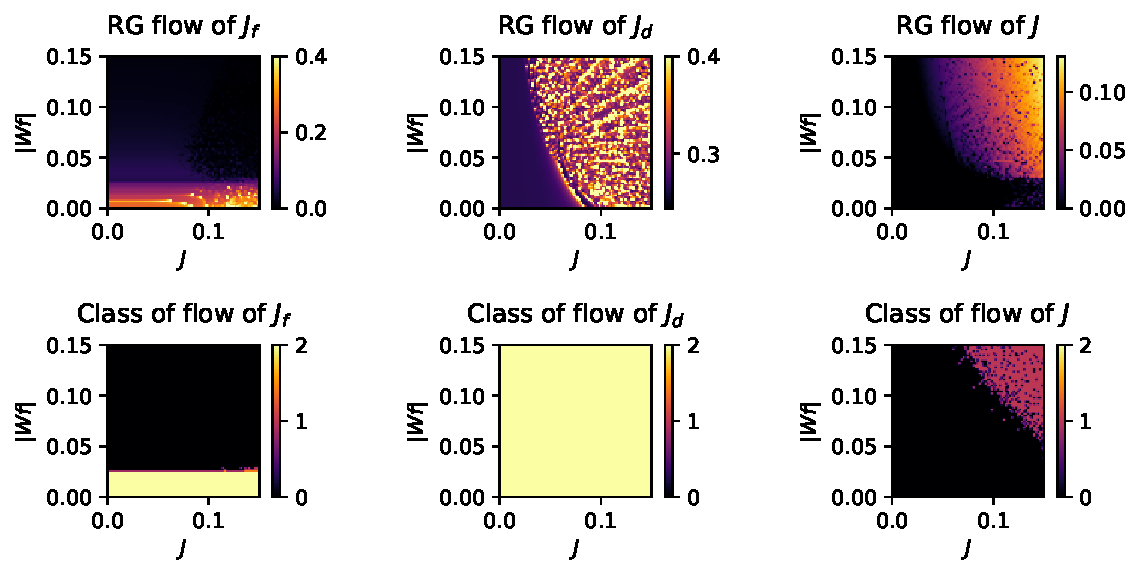
\includegraphics[width=\textwidth]{bilayerHubbard.pdf}

\section{RG flow simulation on the 2D square lattice}
Kondo coupling and bath interaction acquire \(k-\)dependence:
\begin{equation}\begin{aligned}
	J({\bf k}, {\bf q}) &= \frac{J}{2}\left[\cos({\bf k}_x - {\bf q}_x) + \cos({\bf k}_y - {\bf q}_y)\right]~,\\
	W({\bf k}, {\bf q}, {\bf k}^\prime, {\bf q}^\prime) &= \frac{W}{2}\left[\cos({\bf k}_x - {\bf q}_x + {\bf k}^\prime_x - {\bf q}^\prime_x) + \cos({\bf k}_y - {\bf q}_y + {\bf k}^\prime_y - {\bf q}^\prime_y)\right]~.
\end{aligned}\end{equation}
The particle-hole transformed state \(\bar{\bf q}\) associated with \({\bf q}\) is defined as \(\bar {\bf q} = {\bf q} + \left(\pi, \pi\right)\) if \({\bf q}\) is in the first or third quadrant and \({\bf q} + \left(\pi, -\pi\right)\) is in the second or fourth quadrant.

We first introduce a non-zero chemical potential in the conduction bath of the two layer:
\begin{equation}\begin{aligned}
	H_\text{aux} &= \sum_{{\bf k},\sigma,\alpha}\left(\epsilon_{{\bf k},\alpha} - \mu\right)n_{{\bf k},\sigma,\alpha} + \sum_\alpha\sum_{Z \in \text{NN}}\left[\frac{1}{2}J_\alpha\sum_{\sigma,\sigma^\prime}{\bf S}_\alpha \cdot {\boldsymbol{\sigma}}_{\alpha\beta}c^\dagger_{Z,\sigma,\alpha}c_{Z,\sigma^\prime,\alpha} - \frac{W_\alpha}{2} \left(n_{Z,\uparrow,\alpha} - n_{Z,\downarrow,\alpha}\right)^2\right] + J{\bf S}_f \cdot {\bf S}_d~.
\end{aligned}\end{equation}
The effect of this is to split the RG equation into contributions from particle and hole sectors:
\begin{equation}\begin{aligned}
	&\frac{\Delta J_\alpha}{\Delta D} =\\
	& \frac{1}{2}\int_{PS} d{\bf q} ~\rho({\bf q}) \left[J_\alpha({\bf k}_1, {\bf q})J_\alpha({\bf q}, {\bf k}_2) + J_\alpha({\bf q}, \bar {\bf q})W_\alpha({\bf k}_1, {\bf q}, \bar {\bf q}, {\bf k}_2)\right]\left(\frac{1/4}{1/G_\alpha^{(0)}({\bf q}) + \mu/2 + 3J/4} + \frac{3/4}{1/G_\alpha^{(0)}({\bf q}) + \mu/2 - J/4}\right)\\
									  &+ \frac{1}{2}\int_{HS} d{\bf q} ~\rho({\bf q}) \left[J_\alpha({\bf k}_1, {\bf q})J_\alpha({\bf q}, {\bf k}_2) + J_\alpha({\bf q}, \bar {\bf q})W_\alpha({\bf k}_1, {\bf q}, \bar {\bf q}, {\bf k}_2)\right]\left(\frac{1/4}{1/G_\alpha^{(0)}({\bf q}) - \mu/2 + 3J/4} + \frac{3/4}{1/G_\alpha^{(0)}({\bf q}) - \mu/2 - J/4}\right)~,
\end{aligned}\end{equation}
where \(PS\) and \(HS\) integrate over the particle and hole sectors of the excited states (where the excited states are occupied and unoccupied respectively).

Since the bath interaction doesn't renormalise, it's functional form remains unchanged and can be substituted into the RG equations. In fact, we can write the expressions in a compact matrix form for efficient computation:
\begin{equation}\begin{aligned}
	\frac{\Delta J_\alpha}{\Delta D} = J_\alpha \mathcal{G}_\alpha J_\alpha^\dagger + \mathcal{W}_\alpha\text{Tr}\left[\mathcal{G}^\prime_\alpha\right]~,
\end{aligned}\end{equation}
where all objects are matrices. \(J_\alpha\) is the Kondo coupling matrix. \(\mathcal{G}_\alpha\) is a diagonal matrix with matrix elements 
\begin{equation}\begin{aligned}
\mathcal{G}_\alpha[q, q] = \begin{cases}
	\rho(q) \left(\frac{1}{8}\frac{1}{1/G_\alpha^{(0)}({\bf q}) + \mu/2 + 3J/4} + \frac{3}{8}\frac{1}{1/G_\alpha^{(0)}({\bf q}) + \mu/2 - J/4}\right),~{\bf q}\in\text{PS}~,\\
\rho(q) \left(\frac{1}{8}\frac{1}{1/G_\alpha^{(0)}({\bf q}) - \mu/2 + 3J/4} + \frac{3}{8}\frac{1}{1/G_\alpha^{(0)}({\bf q}) - \mu/2 - J/4}\right),~{\bf q}\in\text{HS}~~,
\end{cases}
\end{aligned}\end{equation}
if \(q\) is in the UV subspace and zero otherwise. \(\mathcal{W}_\alpha\) is the bath interaction matrix whose matrix elements are given by \(\mathcal{W}_\alpha[k, k^\prime] = \frac{W}{2}\left[\cos(k_x - k^\prime_x) + \cos(k_y - k^\prime_y)\right]\). Finally, \(\mathcal{G}^\prime_\alpha\) is another diagonal matrix whole matrix elements are defined as \(\mathcal{G}^\prime_\alpha[q,q] = \mathcal{G}[q, q] J_\alpha[q,\bar q]\).

The RG equation for the inter-layer coupling \(J\) can be written as
\begin{equation}\begin{aligned}
	\frac{\Delta J}{\Delta D} &= \frac{1}{2} {\bf J} \cdot \mathcal{\bf G}~,
\end{aligned}\end{equation}
where \({\bf J}\) and \(\mathcal{\bf G}\) are vectors defined by the elements \({\bf J}[q] = J_f(\bar{\bf q},{\bf q}) J_d({\bf q},\bar{\bf q})\) and 
\begin{equation}\begin{aligned}
	\mathcal{\bf G}[q] = \rho({\bf q}) \left[\frac{1}{\omega - \frac{1}{2}\bar\epsilon_f({\bf q}) + \frac{1}{2}J_f({\bf q}) + W_f({\bf q}) - \frac{1}{4}J} + \frac{1}{\omega - \frac{1}{2}\bar\epsilon_d({\bf q}) + \frac{1}{2}J_d({\bf q}) + W_d({\bf q}) - \frac{1}{4}J}\right]~.
\end{aligned}\end{equation}

\end{document}
